
\documentclass[14pt, english]{article}

\title{{\bf Travelling Salesman Problem (TSP)}}
\author{Louise Ruth Harding \\ Robin Khatri \\ Laetitia Couge\\ Mohammed Paul Doust \\ Mohammed Nassar}

\date{\today}


\usepackage[T1]{fontenc}
\usepackage{babel}
\usepackage{geometry}
\usepackage{titling}
\usepackage{hyperref}
\usepackage{graphicx}
\usepackage{float,flafter}
\renewcommand\maketitlehooka{\null\mbox{}\vfill}
\renewcommand\maketitlehookd{\vfill\null}
\usepackage{blindtext}
\usepackage[utf8]{inputenc}
\usepackage{algorithm}
\usepackage{algorithmic}
\usepackage[absolute,overlay]{textpos}
\usepackage{graphicx}
\setlength{\droptitle}{-4em}     % Eliminate the default vertical space
\addtolength{\droptitle}{-4pt}   % Only a guess. Use this for adjustment
\usepackage[export]{adjustbox}
\usepackage{amsmath}
\usepackage{caption}
\usepackage{subcaption}
\usepackage{subfiles}
\begin{document}
\newcommand\tab[1][1.2cm]{\hspace*{#1}}

\begin{titlingpage}
\maketitle
\center 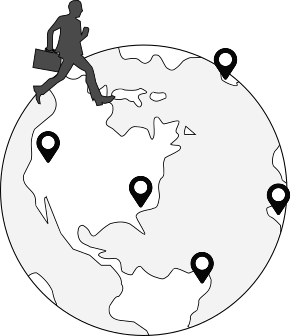
\includegraphics[scale=0.5]{tsp.png}

\end{titlingpage}
\tableofcontents
\newpage

\section{Introduction}

Consider a salesman who has to visit a set of cities and return to the city he started from provided he visitseach city only once.\\
\\
\noindent
The problem is to minimize the total cost or distance of the route. This is known as the Travelling Salesman Problem.\\
\\
\noindent
The problem can be summarised as follows: \\
\\
\tab TSP = $\{(G,f,t)$: $G = (V,E)$ is a complete graph,\\
\tab \tab $f$ is a function $V\times V \rightarrow Z,$\\
\tab \tab $t \in Z,$ \\
\tab \tab $G$ is a graph that contains a travelling salesman tour with costs or distances that\\ \tab \tab does not exceed $t\}$.

\subsection{Symmetric Travelling Salesman Problem}

If in a travelling salesman problem, cost or distance of travelling from city $i$ to city $j$ is equal to the cost or distance of travelling from city $j$, $i.e.$ the cost matrix is symmetric, then the problem is said to be \emph{Symmetric Travelling Salesman Problem}.

\subsection{Asymmetric Travelling Salesman Problem}

If in a travelling salesman problem, cost or distance of travelling from city $i$ to city $j$ can differ from the cost or distance of travelling from city $j$, $i.e.$ the cost matrix is asymmetric, then the problem is said to be \emph{Asymmetric Travelling Salesman Problem}. A real world example could be routes consisting of some one-way roads.


\subsection{Sparsity of TSP}
\newpage
\section{Brute Force Algoritm}
\subsection{Introduction}
Bruteforce algorithm runs through all possible solutions and selects the best one. It is not an optimal algorithm to use for TSP with a large number of nodes.

\subsection{Experiment and complexity}

We tested the code on both symmetric and asymmetric problems. Since it provides exacts solutions, the solutions were optimal.\\

\noindent
The complexity of the algorithm is $\mathcal{O}(n!)$. We tested it on tsp's upto 10 cities, as the complexity increased rapidly after that.

\begin{center}
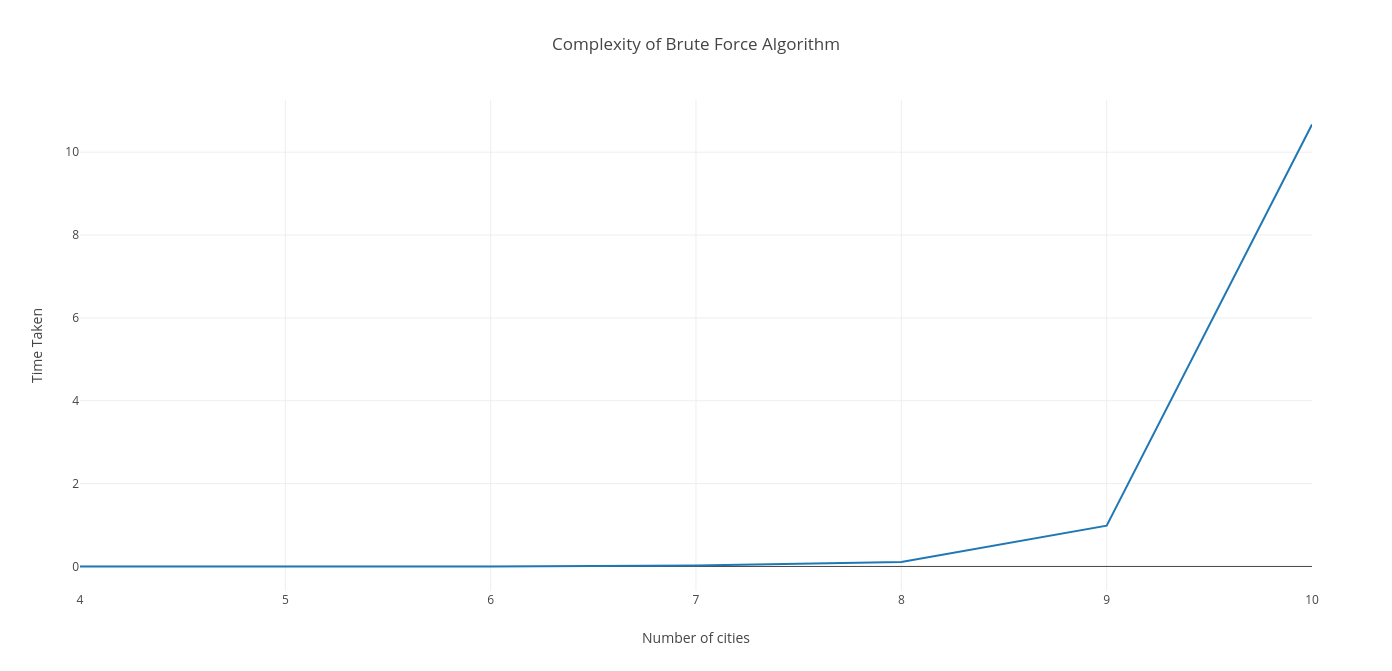
\includegraphics[scale=0.3]{bruteforce.png}
\end{center}

\noindent
In case of Symmetric TSPs, the computational time can be reduced by computing distances only for permutations which begin with our choice of first city. However, the complexity still remains $\mathcal{O}(n!)$, but number of permutations to cover decrease.\\
\\
\noindent
Improvements on Bruteforce Algorithm are provided with Branch and Bound Algorithms presented in the next section.

\newpage
\section{Branch and Bound With Adding and Removing Edges}
\subsection{Introduction}
One of the strategies used for searching the solution space is Branch and Bound keep dividing the space into branches. one for solutions containing a given edge and the other for those excluding the given edge. forming a binary tree as follows:
\newline \newline
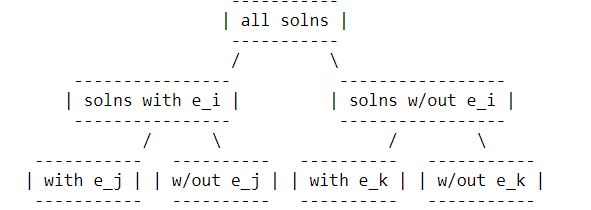
\includegraphics[width=\textwidth] {solution-tree.jpg}
\newline \newline
The main parts of these algorithm are:
\begin{enumerate}
    \item Bounding Function
    \item Choosing Splitting Edge
    \item How to Include Edge
    \item How to Exclude Edge
\end{enumerate}

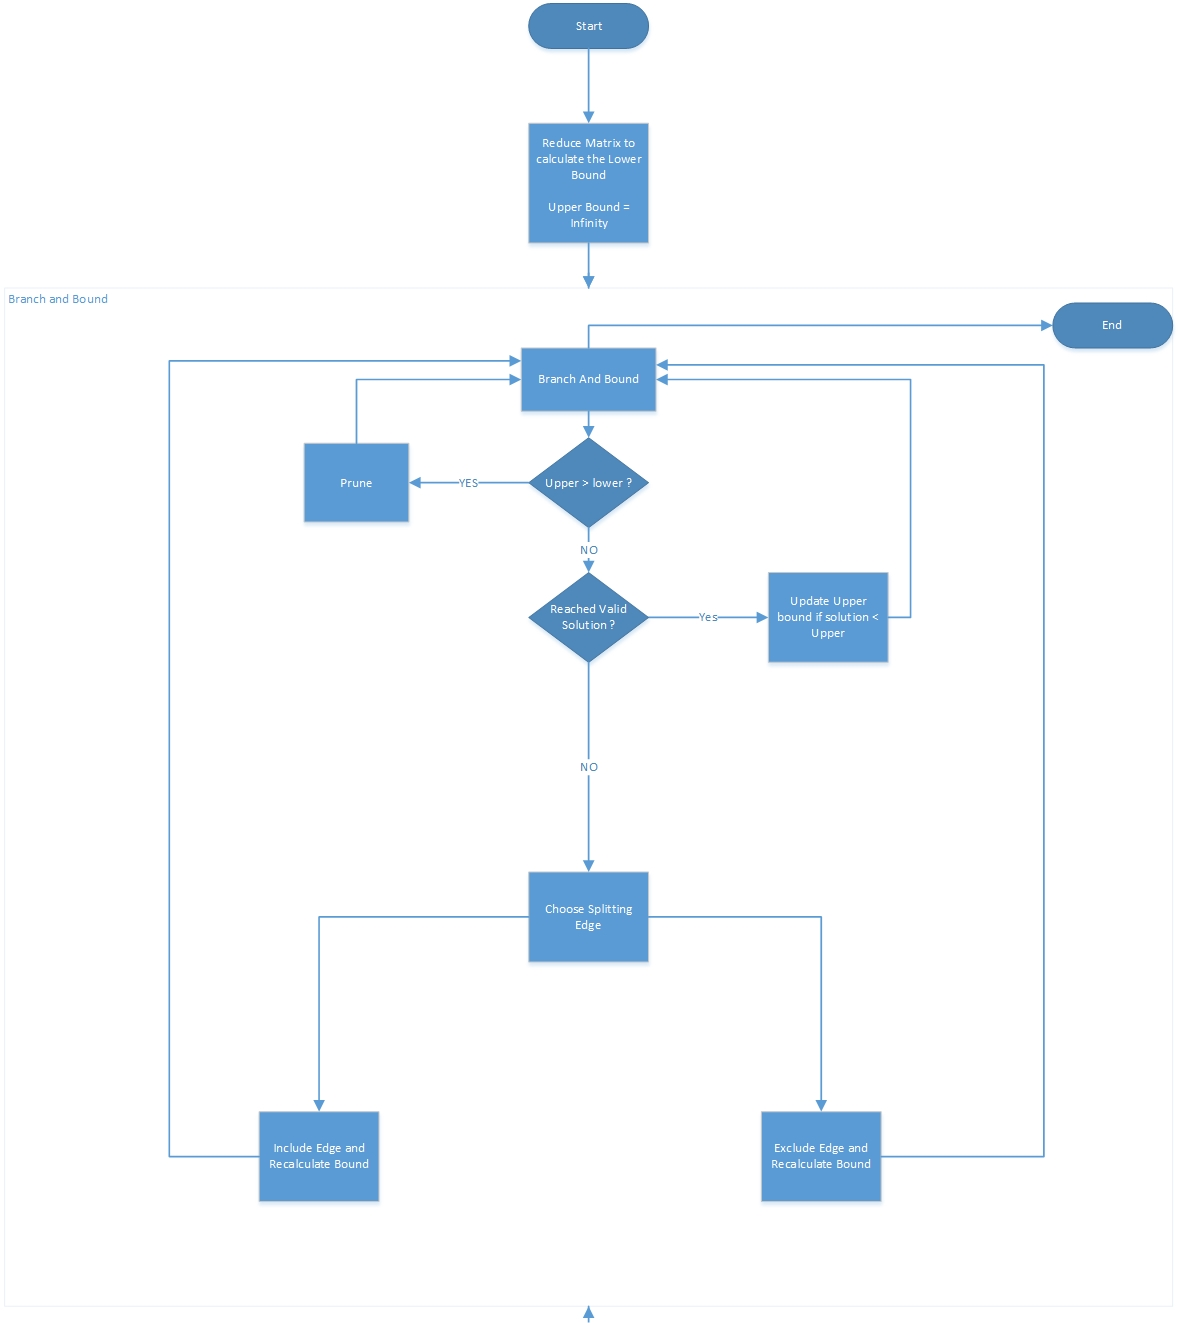
\includegraphics[width = \textwidth]{bnb-flow.jpg}

\newpage
\subsection{Bounding Function (Reduction)}
The solution is bounded by normalizing the solution matrix. this is done by reducing the rows first and the columns after.
by reducing the Rows/Columns we mean normalizing them. we subtract the minimum element from each row from each element at that row. and the same for columns. at the end we will have a matrix with at least one zero in each column and each row.
Our lower bound will be the sum of all minimum values with used to reduce the matrix.

\subsection{Choosing Splitting Edge}
We are looking to maximize the right part by trying to raising the lower bound of the right sub-tree. In order to do that, we choose to split on the edge that best maximize the lower bound. We look for the zero weight edges that maximize the increasing in the lower bound.

\subsection{How to Include Edge}
Including an edge (ie, I -> J) is done by first, forbidding the going back from J -> I by setting the weight of edge J -> to INFINITY ( we also forbid the going back to any sub-path in our partial solution). Moreover, since we have used this edge, we cannot go from node i to any other node, and similarly, we cannot reach node J. Consequently, we delete the I th row and the J th column from our solutions matrix.
in the end, we reduce the new matrix after including the edge.

\subsection{How to Exclude Edge}
To exclude edge (ie, I-> J), we start by setting the cost of the edge I->J to INFINITY. and we reduce the new matrix afterwards.

\subsection{Complexity}

\begin{center}
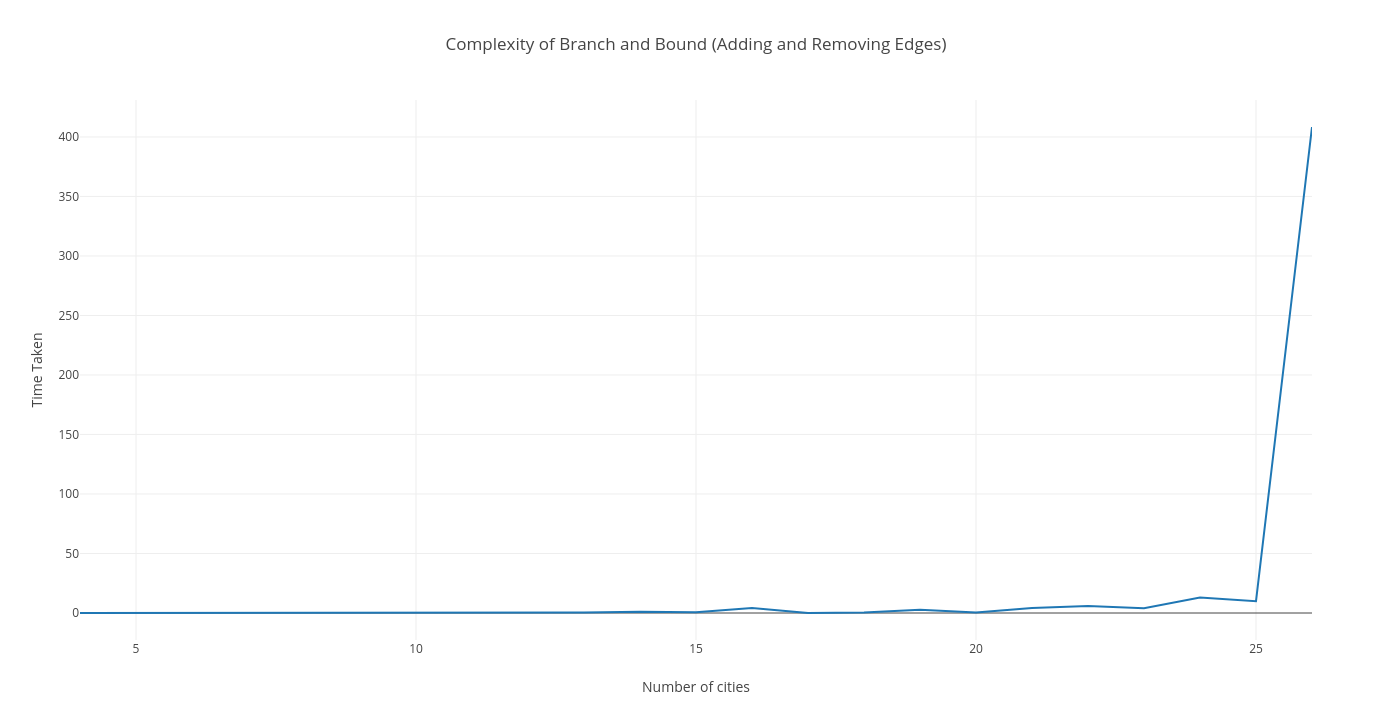
\includegraphics[scale=0.3]{branchandbound.png}
\end{center}
\newpage

\section{Randomized algorithm}
\subfile{algo_random}

\section{Dynamic Programming algorithm}
\subfile{algo_dp}

\section{Ant Colony Algorithm}

\subsection{Introduction}

Ant Colony Algorithm is a probabilistic algorithm that takes inspiration from the behavior of ants to Travelling Salesman Problems. The first algorithm that took inspiration from ants was described in 1992 by Marco Dorigo in his PhD thesis. Later, there has been various optimization techniques building upon this research. In 2004, book titled Ant Colony Optimzation was published. We took inspiration from this book for our implementation of Ant Colony Algorithm.

\subsection{Behavior of Ants}

\begin{center}
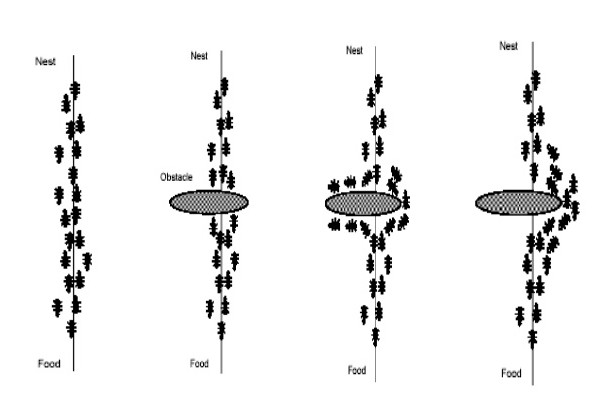
\includegraphics[scale=0.5]{antfood.jpg}
\end{center}

Ants live together in colonies and they form a highly structured societies. Ants do not have a developed visual skills and some of the species of ants are blind. They, however, make use of pheromones which they leave behind while naviagting. This is a form of indirect communication with other ants in the colony. Due to high concentration of pheromones on a path, ants are influenced to take the path previously travelled by the former ants. This behavior leads to the convergence of establishing a path, \emph{i.e.} after a certain time, all the ants which are travelling together follow the same path (and find the food!)
 
\subsection{Theory}

The behavior of ants described above can be utilised to form an algorithm able to provide approximate solutions to TSP problems.\\

\noindent
Consider $m$ ants and they are placed in $n$ cities chosen randomly from the list of cities in our problem.\\
\\
\begin{center}
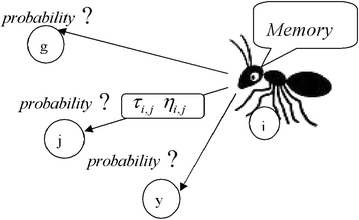
\includegraphics[scale=0.5]{ant.png}
\end{center}

\noindent
Ant number $k$ moves from city $i$ to city $j$ with probability $p_{ij}^m$ given below:

\begin{center}
$p_{ij}^k = \frac{{(\tau_{ij}^\alpha)(\eta_{ij}^\beta)}}{\sum_{ij \rightarrow allowed}{(\tau_{ij}^\alpha)(\theta_{ij}^\beta)}}$
\end{center}
\noindent
Where, $\tau_{ij}$ is the amount of pheromone deposited for transition from city \emph{i} to \emph{j}.

\tab  $\eta _{ij}$ is the desirability of going to city ${j}$ from city ${i}$. It is given by ${1/d_{ij}}$.

\tab $\alpha$ and $\beta$ are parameters that respectively control the influence of $\tau_{ij}$ and $\eta _{xy}$.\\

\noindent
Many special cases of Ant Colony Optimzation has been proposed. In this project, we have considered Ant Colony System (ACS). Other popular approaches are Ant System (Earliest Ant Colony Algorithm) and MAX-MIN Ant System (MMAS). These Optimization methods differ in their approach of updating pheromones and calculating transition probabilities $p_{ij}$. \\
\\
\noindent
{\bf Ant System (AS)}:\\
\\
In AS,\\
\noindent
Updates of pheromones:\\ 
When all ants complete their tours, trails of pheromones are updated as follows:

\begin{center}
$\tau_{ij} = (1-\rho).\tau_{ij} + \sum_{k}\Delta \tau_{ij}^k$
\end{center}
where $\Delta \tau_{ij}^k$ can be calculated depending upon the strategy we choose, and $\rho$ is the evaporation rate. Higher the $\rho$, quicker is the evaporation rate of pheromones.\\
\begin{center}
$\Delta \tau _{ij}^{k}={\begin{cases}Q/L_{k}&{\mbox{if ant }}k{\mbox{ uses transition city }}i \rightarrow j{\mbox{ in its tour}}\\0&{\mbox{otherwise}}\end{cases}}$\\
\end{center}
\noindent
Where $L_{k}$ is the cost of ant k's tour, and Q is a constant.\\

\noindent
{\bf Ant Colony System (ACS)}: \\
\\
In ACS,\\
The local pheromone update is done by each ant k after every transition $i \rightarrow j$. Each ant applies this update to the last edge it transversed.
\begin{center} {$\tau_{ij} = (1-\phi).\tau_{ij} + \phi.\tau_{0}$} \end{center}
Where $\tau_{0}$ is the initial value of the phreromone (Usually kept small) and $\phi$ is the pheromone decay coefficient. After a complete travel, the local updates are deleted.\\

\noindent
Secondly, after all ants have completed the paths, the global update of pheromone is done only taking into account the best tour so far. In this case, 

\begin{center}
$\tau_{ij} = (1-\rho).\tau_{ij} + \Delta \tau_{ij}^{best}$
\end{center}
\noindent
Where,
\begin{center}
$\Delta \tau _{ij}^{best}={\begin{cases}Q/L_{Best}&{\mbox{if best ant}}{\mbox{ uses transition city }}i \rightarrow j{\mbox{ in its tour}}\\0&{\mbox{otherwise}}\end{cases}}$\\
\end{center}
\noindent
$L_{Best}$ is the total length of the best path so far, and Q is a constant.\\
 
\subsection{Algorithm}

\begin{enumerate}
	\item Initialize parameters
	\item Randomly place m ants in n cities
	\item Choose transitions
	\begin{enumerate}
		\item Calculate $p_{ij}$ using equation given above. 
		\item trasit from city {i} to {j} randomly based on probabilities $p_{ij}$ and locally update pheromones
	\end{enumerate}	 
	\item When all ants have completed a solution, choose best solution and globally update pheromones using aforementioned expressions and remove local updates
	\item Iterate the process
\end{enumerate}

\subsection{Results on TSPLIB Problems}
We chose $\alpha$ to be 1 and $\beta$ to be 10. We have no experimented with other values of these parameters, however, there is literature suggesting choice of these hueristics but solutions were close to optimal. Choice of number of ants depend on the number of cities in our problem. In general we considered number of ants to be close to the number of cities. \\ 
\\
In our experiments, number of ants were chosen to be in a range of [10,50], and number of iterations we chose to run our algorthim for was in a range of (100-500).\\
\\
We considered both Symmetric and Assymetric TSP Problems from TSPLIB database, and solutions are presented below:

\begin{table}[h!]
  \begin{center}
    \caption{Observed vs Optimal solutions}
    \label{tab:table1}
    \begin{tabular}{c|c|c|c|c|c}
      \textbf{Dataset} & \textbf{No. of cities} & \textbf{No. of ants} & \textbf{Iterations} & \textbf{Solution found}  &\textbf{Opt. solution}\\ % 
      \hline
      {burma14.tsp} & 14 & 30 & 500 & 3336 & 3323 \\ % <--
      {ulysses16.tsp} & 16 & 15 & 800 & 6859 & 6859 \\ 
	 {att48.tsp} & 48 & 50 & 500 & 10725 & 10628 \\ % <--
	 {berlin52.tsp} & 52 & 20 & 100 & 7894 & 7542 \\ % <--
	 {ch150.tsp} & 150 & 50 & 500 & 10725 & 10628 \\ % <--
	 {gr124.tsp} & 124 & 50 & 500 & 10725 & 10628 \\ % <--
	 {d657.tsp} & 48 & 50 & 500 & 10725 & 48912 \\ % <--
	 {st70.tsp} & 70 & 10 & 100 & 670 & 705 \\ % <-- 
	 {gr17.tsp} & 17 & 15 & 500 & 2164 & 2085 \\ % <--
	 {gr24.tsp} & 24 & 20 & 500 & 1345 & 1272 \\ % <--
	 {gr48.tsp} & 48 & 50 & 500 & 5280 & 5046 \\ % <--
	 {gr96.tsp} & 96 & 50 & 500 & 10725 & 10628 \\ % <--
	 {rat195.tsp} & 195 & 50 & 500 & 10725 & 10628 \\ % <--
	 {br17.atsp} & 17 & 50 & 500 & 10725 & 39 \\ % <--
	 {ft70.atsp} & 70 & 50 & 500 & 10725 & 38673 \\ % <--
	 {ftv47.atsp} & 47 & 50 & 500 & 10725 & 10628 \\ % <--
	 {ftv64.atsp} & 64 & 50 & 500 & 10725 & 10628 \\ % <--
	 {ftv33.atsp} & 33 & 50 & 500 & 10725 & 10628 \\ % <--
	 {ftv38.atsp} & 38 & 50 & 500 & 10725 & 10628 \\ % <--
	 {kro134p.atsp} & 134 & 50 & 500 & 10725 & 10628 \\ % <--
	 {ry48p.atsp} & 48 & 50 & 500 & 10725 & 10628 \\ % <--
	 {rbg323.atsp} & 323 & 50 & 500 & 10725 & 10628 \\ % <--
	 
    \end{tabular}
  \end{center}
\end{table}
\newpage
\noindent
{\bf Selection of parameters}:\\
\\
\noindent
Complexity of ant colony system (ACS) method is quite high, especially for problems with hundereds of cities. The reason being essentially two loops in every pheromone update. This can be improved using further optimisation methods \emph{e.g} nearest neighbour search and 3-OPT methods. These optimizations are suitable for TSPs of large sizes.\\
\\
\noindent
Graph below shows the evolution of computational time with increasing size and sparsity of TSP.


\newpage
\section{Genetic Algorithm}
\subsection{Introduction}
We present in this report the main description for the attached source code to solve Travelling salesman Problem. \newline \newline
As illustrated in the figure below, the main algorithm pipeline contains several main components:
\begin{enumerate}
    \item Initializing Algorithm Parameters
    \item Generate Initial Population
    \item Fitness Evaluation
    \item Parents Selection
    \item Crossover
    \item Mutation
    \item Generate New Population
\end{enumerate}
The following sections will explain briefly each components.
\newline \newline
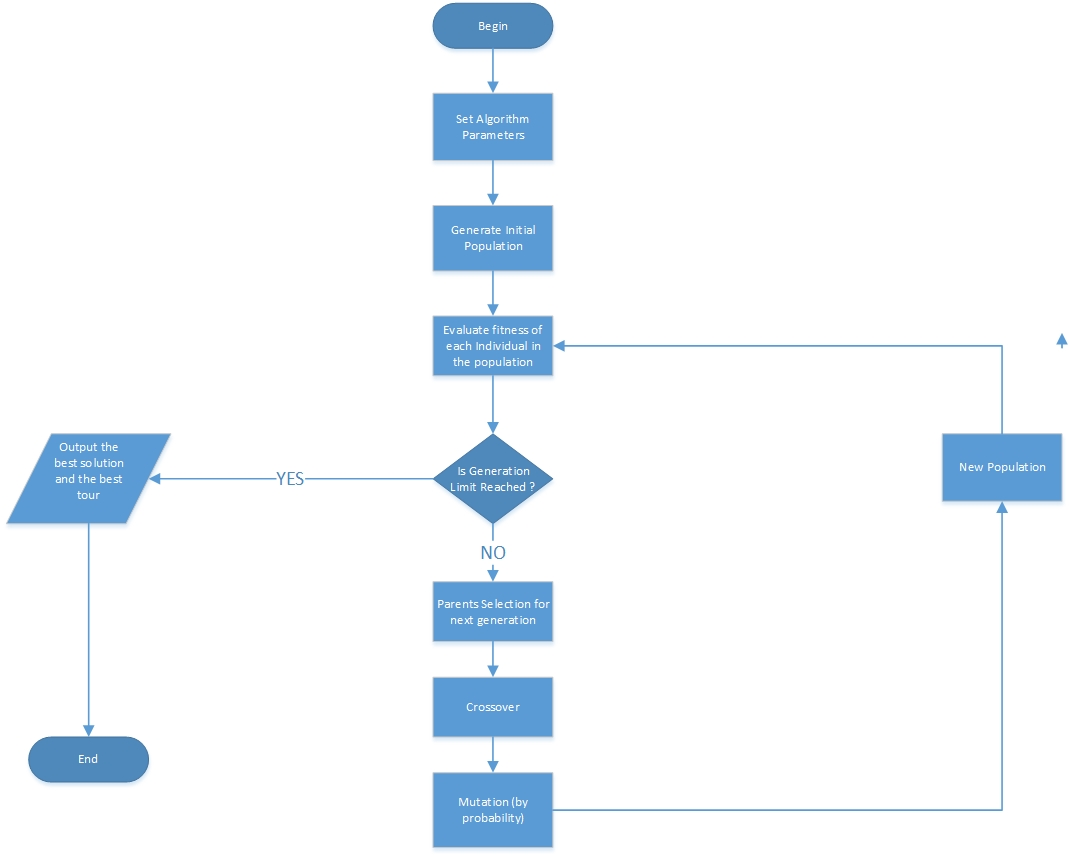
\includegraphics[width=\textwidth]{tsp-genetic-flowchart.jpg}

\subsection{Initializing Algorithm Parameters:}
In this step, several parameters should be initialized by the user. Specifically, \begin{enumerate}
    \item Max Population Size: 
    to specify the maximum number of individuals in any population
    \item Max Generation Numbers: usually the termination condition
    \item Mutation Rate: a real number in [0,1] specify the likelihood of mutation to happen
\end{enumerate}

\subsection{Generate Initial Population:}
In this step an initial generation is created randomly by creating a first random individual (Tour), and use shuffling on this individual until we reach the max population size. 
\subsection{Fitness Evaluation for Elitism:}
in this step, the fitness function for each individual should be calculated. For the TSP problem. the fitness function could be define as the total sum of distances for each tour.
This fitness function is used to evaluate how good each individual (Solution). Consequently, the fittest individual is elited to the next generation directly.
\subsection{Parents Selection:}
In this step, parents are chosen to mate together (crossover) and have a new individual. the selection process could be done in several ways. we applied Roulette Selection (with flexibility in the code to add new other selection algorithms without changing the code).
the basic of Roulette Selection is to pick a parent randomly according to weighted probability for each individual. the weights here represented by the fitness of the individual. In other words, individuals with high fitness function, have higher probabilities to be selected.
\subsection{Crossover:}
The crossover is the process of merging two individuals to have a new ones. there is several ways to implement the crossover. in our case, we implemented the Single Point Crossover. where a random point is generated bounded by the length of the solution. Afterwards, a new individuals are generated by taking the first part (before the picked point) from the first parent and the rest from the other taking into account the satisfaction of TSP constraints (no duplication) 
\subsection{Mutation:}
Each individual might undergo a mutation with a probability (specified in the parameters). the mutation basically is done by scanning the individual genes and picking a random number (bounded by the length of tour) and swap the current gene with the randomly picked one.
\subsection{Generate New Population:}
We keep repeating steps 5,6,7 until we have a full new population (enhanced one). and we go back to step 4 while we have not reached the generation limit.

\subsection{Complexity}

\begin{center}
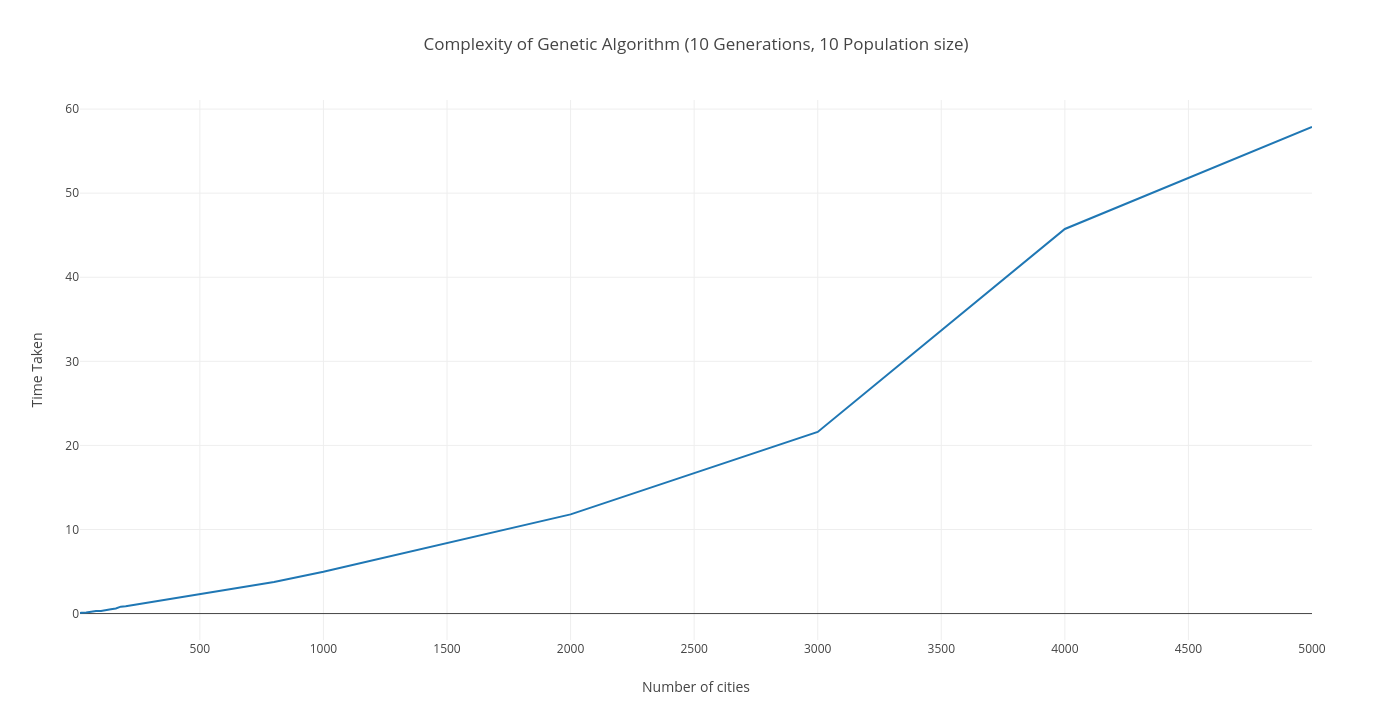
\includegraphics[scale=0.3]{genetic1.png}
\end{center}

\begin{center}
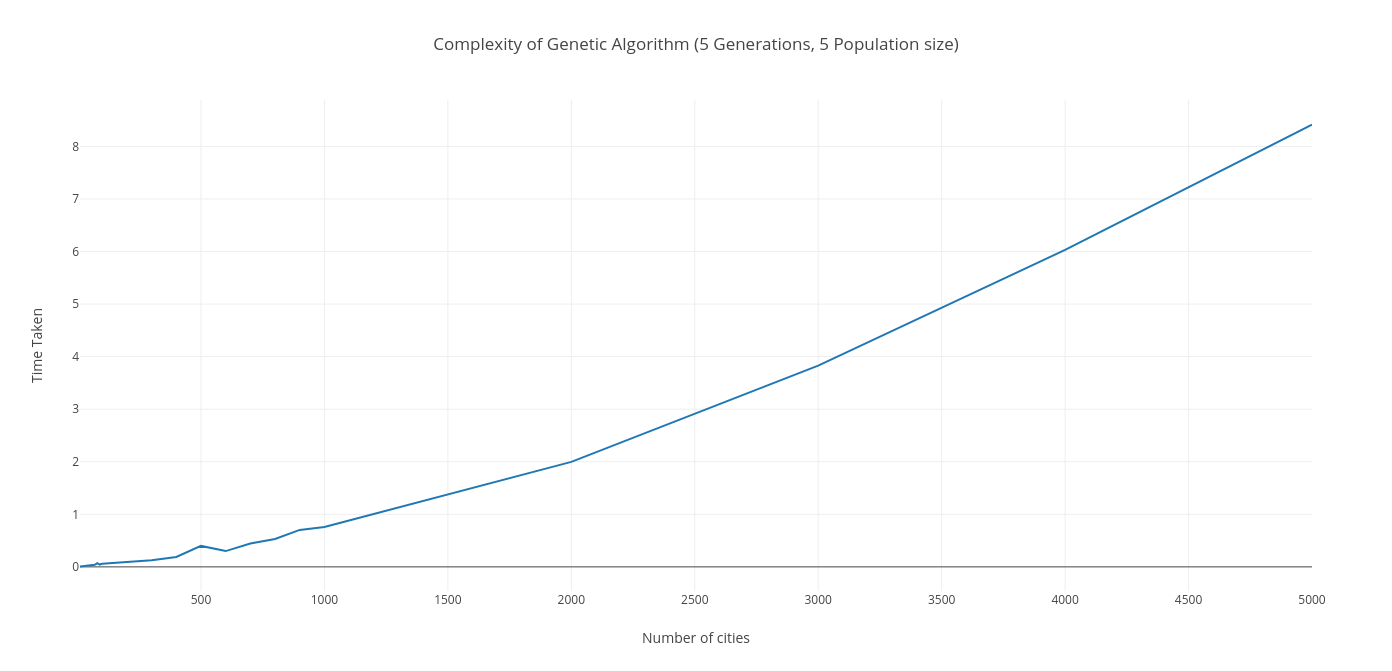
\includegraphics[scale=0.3]{genetic2.png}
\end{center}

\begin{center}
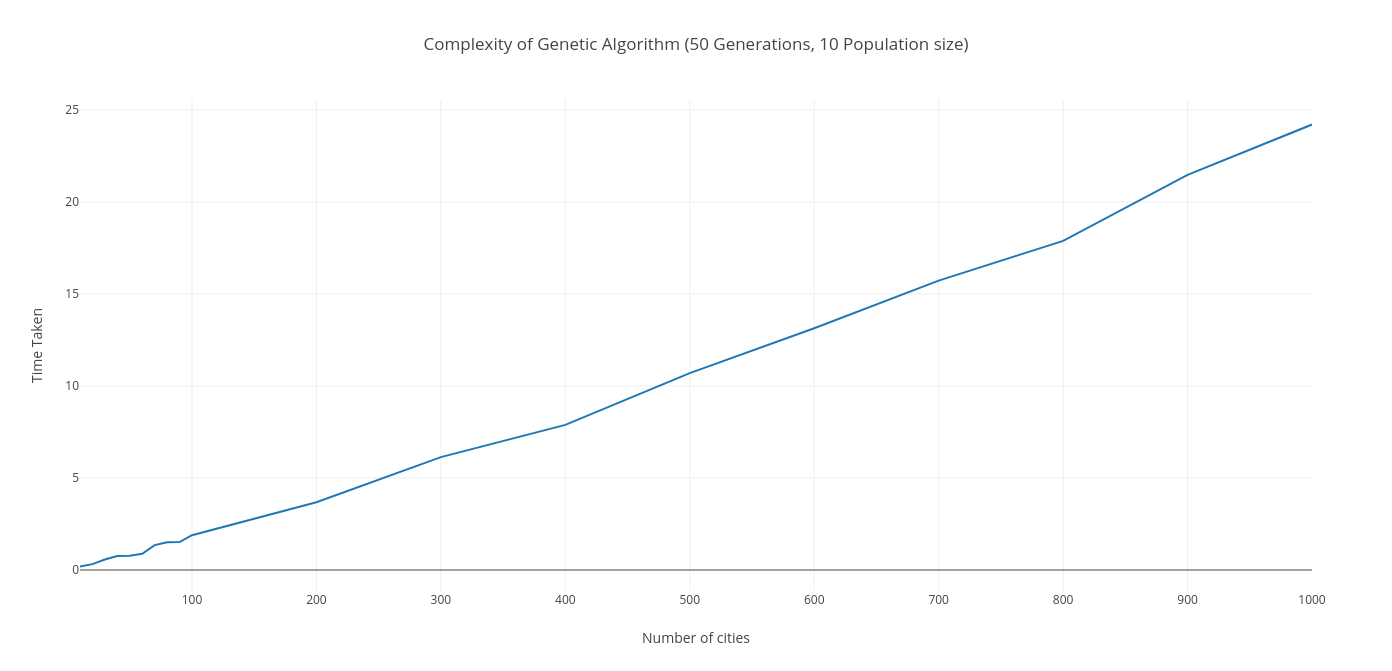
\includegraphics[scale=0.3]{genetic3.png}
\end{center}

\end{document}  